\documentclass[a4paper,oneside]{article}
\usepackage{phd}
\usepackage{hyperref}
\makeatletter
\cxset{plain sections/.style={
 chapter name = CHAPTER,
 chapter toc = true,
 chapter color= thegray,
 chapter opening = right, 
 chapter numbering = arabic,
 chapter font-family= sffamily,
 chapter font-weight= bold,
 chapter font-size= LARGE,
 chapter before={\thinrule\vspace*{20pt}\par\hfill\hfill},
 chapter after={\vskip0pt\par},
 chapter spaceout = soul,
 number font-size= Large,
 number font-family= rmfamily,
 number font-weight= bfseries,
 number color=thegray,
 number before=\vspace*{5pt}\hfill\hfill,
 number dot=.,
 number after={\hspace*{7pt}\par},
 title beforeskip={\vspace*{10pt}},
 title afterskip={\vspace*{50pt}\par},
 title before={\hfill\hfill\raggedleft},
 title after={\par\thinrule},
 title font-family=\sffamily,
 title font-color= teal,
 title font-weight=\bfseries,
 title font-family=\sffamily,
 title font-size= Large,
 title font-shape= upshape,
 title spaceout= none,
 title beforeskip={\vspace*{10pt}},
 title afterskip={\vspace*{50pt}\par},
 title before={\hfill\hfill\raggedleft},
%
% numbers
% number font-family=\sffamily,
% number font-weight=\bfseries,
 number color=thelightgray,
 number before=\par\vspace*{5pt}\hfill\hfill,
 number dot=,
 number after={\hspace*{7pt}\par},
 number position=rightname,
 section color= thered,     
 section beforeskip=15pt,
 section afterskip=15pt,
 section indent=0pt,
 section font-family= sffamily,
 section font-size= LARGE,
 section font-weight= bfseries,
 section font-shape=,
 section align= centering,
 section numbering prefix =,%use \thechapter. for books or add as option
 section numbering= arabic,
 section spaceout=none,
 section number after=ooo,
 subsection color= thered,
       subsection beforeskip=10pt,
       subsection afterskip=10pt,
       subsection indent=0pt,
       subsection font-family= rmfamily,
       subsection font-size= large,
       subsection font-weight= bold,
       subsection font-shape= upshape,
       subsection align= centering,
       subsection numbering prefix=\thesection.,%\S\hairsp,%add . 
       subsection numbering custom =\@arabic\c@subsection,% \two@digits{\@arabic\c@subsection},%
       subsubsection color= gray,
       subsubsection beforeskip=5pt plus3pt minus 2pt,
       subsubsection afterskip=5pt,
       subsubsection indent=0pt,
       subsubsection font-family= rmfamily,
       subsubsection font-size= normalfont,
       subsubsection font-weight= bold,
       subsubsection font-shape= itshape,
       subsubsection align= centering,
       subsubsection numbering prefix =\thesubsection.\@arabic\c@subsubsection,
       subsubsection numbering custom =, %\two@digits{\@arabic\c@subsubsection},
       subsubsection number after =, 
%
       paragraph color= thegrey,
       paragraph beforeskip=,
       paragraph afterskip=-0.5em,
       paragraph indent=0pt,
       paragraph font-family= rmfamily,
       paragraph font-size= large,
       paragraph font-weight= bfseries,
       paragraph font-shape=,
       paragraph align= centering,
       paragraph number after = 0pt,
       paragraph numbering=numeric,
       subparagraph color= thered,
       subparagraph beforeskip=0pt,
       subparagraph afterskip=-.5em,
       subparagraph indent=0pt,
       subparagraph font-family= sffamily,
       subparagraph font-size= large,
       subparagraph font-weight= normalfont,
       subparagraph font-shape= slshape,
       subparagraph align= RaggedRight,
       subparagraph number after =, % can affect all needs checking
       %subsubsection numbering prefix=\S\hairsp\thesection,%add . here if need be
       subparagraph numbering=none,
}
}
\cxset{plain sections}
\cxset{style13/.style={
 name= {\protect\pan अमुकग्रन्थे},
 chapter spaceout = none,
 numbering=arabic,
 number font-size= HUGE,
 number font-family= sffamily,
 number font-weight= bfseries,
 number color= gray!50,
 number before=\par\vspace*{5pt}\hfill\hfill,
 number dot=,
 number after={\hspace*{7pt}\par},
 number position=rightname,
 chapter font-family= sffamily,
 chapter font-weight= bold,
 chapter font-size= LARGE,
 chapter before={\tikzrule\vspace*{20pt}\par\hfill\hfill},
 chapter color= black!50,
 title beforeskip={\vspace*{10pt}},
 title afterskip={\vspace*{50pt}\par},
 title before={\hfill\hfill\raggedleft},
 chapter rule color=teal,
 title after=\par\tikzrule,
 title font-family= sffamily,
 title font-color= teal,
 title font-weight= bfseries,
 title font-size= huge,
 section indent=-1em,
 section align= left,
 section numbering= arabic,
 section indent=0pt,
 section beforeskip=0pt,
 section afterskip= 10pt,
 section color=teal,
 subsection align= ,
 subsection font-family= sffamily,
 subsection font-weight= bfseries,
 subsection color = teal,
 subsection font-size= large,
 subsection font-shape=,
 subparagraph number after=,
 subsubsection align=,
}
}
\cxset{style13}

\renewparagraph
\renewsection
\renewsubsection
\renewsubparagraph
\renewsubsubsection

\makeatother
\newfontfamily\calibri{calibri.ttf}
\begin{document}
\calibri
\lipsum[2]

\bgroup\parindent=0pt
\leavevmode\par
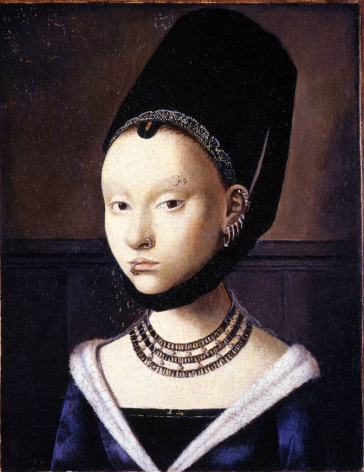
\includegraphics[width=\linewidth]{./images/pierced.png}%
\vskip0sp %
\ifodd\thepage
   %\nobreak
   \hbox to \linewidth{\hfill\scriptsize Credit:\thinspace{\small\itshape Kathleen Gilje}}%
\else
  \nobreak
  \hbox to \linewidth{\scriptsize Credit:\thinspace{\small\itshape Kathleen Gilje}\hfill}%
\fi     
\enlargethispage{30pt}
\nobreak 
\captionof{figure}{Some description of the image.}%
\bigskip
\egroup

\lipsum[1]

\bgroup\parindent=0pt
\leavevmode\par
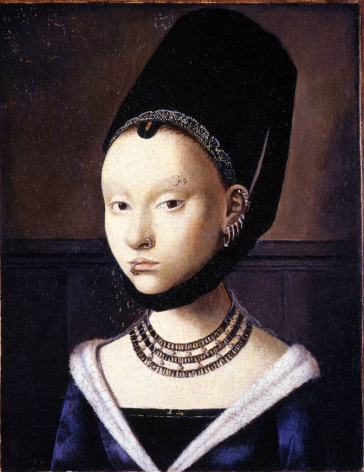
\includegraphics[width=\linewidth]{./images/pierced.png}%
\nobreak
\vskip0sp %
\ifodd\thepage
   \hbox to \linewidth{\hfill\scriptsize Credit:\thinspace{\small\itshape Kathleen Gilje}}%
\else
  \hbox to \linewidth{\scriptsize Credit:\thinspace{\small\itshape Kathleen Gilje}\hfill}%
\fi      
\captionof{figure}{Some description of the image.}%
\bigskip
\egroup

\lipsum[1]

\parindent0pt

\tikzrule

\bgroup
\leftskip-3cm \rightskip2cm
\def\hook{\node[right=5pt, yshift=-12pt] at (0,-3) {\HUGE\color{purple} This is the  Title}; }
\def\hook{}
\makeatletter\@specialtrue 
\cxset{chapter name = CHAPTER}
\expandafter\ifnum\thechapter=0\stepcounter{chapter}\else\fi
\begin{tikzpicture}
%\draw [help lines] (0,0) grid (18,-13);
\draw[fill=red]  (0,0) circle (1.5pt) ;
\node[rectangle,draw, right, baseline] (x) at (0,1) {\LARGE\color{black!30}{before}\relax};
\draw[fill=red]  (0,1) circle (1.5pt) ;
\node[rectangle,draw, right=1sp] at (0,0) {\LARGE\color{black!20} \so\chaptername\relax};

\node[rectangle,draw, color=white, below right, fill=blue!50, text=white] at +(\textwidth+3cm,0) {\scalebox{2}{\HHUGE \thechapter}};
\draw[fill=red]  (0,-3) circle (1.5pt) ;
\node[rectangle, draw, text width=9cm,below right, yshift=-1pt] at (0,-3) {%
         \HUGE Title format\kern0ptt\kern0pting \Large \lorem }; 
\node at (12.5,-9) {\includegraphics[width=7cm]{./images/fashion.jpg}};
\hook
\end{tikzpicture}

\tikzrule 
\egroup

\lipsum
\bigskip

\thispagestyle{empty}


\begin{tikzpicture}
\draw[fill=black!20] (0,0) rectangle (1+1,2) rectangle ++(1+1,-2) {};


\end{tikzpicture}

\end{document}

http://tex.stackexchange.com/questions/48473/best-way-to-give-sources-of-images-used-in-a-beamer-presentation/48479#48479